\documentclass[a4paper, 10pt]{article}
\usepackage{pgf}
\usepackage{eurosym}
\usepackage{graphicx}
\usepackage{wasysym}
\usepackage{hyperref}
\usepackage{listings}
\usepackage{pxfonts}
\usepackage{verbatim}
\usepackage{color}
\usepackage{xcolor}
\usepackage{wrapfig}
\usepackage{enumitem}
\usepackage{booktabs}
\usepackage{tabularx}

\hypersetup{
    bookmarks=true,         % show bookmarks bar?
    unicode=true,          % non-Latin characters in Acrobat’s bookmarks
    pdftoolbar=true,        % show Acrobat’s toolbar?
    pdfmenubar=true,        % show Acrobat’s menu?
    pdffitwindow=true,     % window fit to page when opened
    pdftitle={Assignment 2},    % title
    pdfauthor={Paul Vesey},     % author
    pdfsubject={Construction Project Management},   % subject of the document
    pdfcreator={},   % creator of the document
    pdfproducer={xelatex}, % producer of the document
    pdfkeywords={'Project Management' }, % list of keywords
    pdfnewwindow=true,      % links in new PDF window
    colorlinks=true,       % false: boxed links; true: colored links
    linkcolor=violet,          % color of internal links (change box color with linkbordercolor)
    citecolor=magenta,        % color of links to bibliography
    filecolor=red,      % color of file links
    urlcolor=blue           % color of external links
}

\setlength\parindent{0pt}
\begin{document}

\lstset{language=HTML,
				basicstyle=\small,
				breaklines=true,
        numbers=left,
        numberstyle=\tiny,
        showstringspaces=false,
        aboveskip=-20pt,
        frame=leftline
        }
				
\begin{table}%
	\begin{minipage}{0.4\textwidth}%
			
\includegraphics[width=1\textwidth]{./img/LITlogo.jpg}
	\end{minipage}
	\qquad
	\centering
	\parbox{0.4\textwidth}{
		\begin{large}			
			\begin{tabular}{| r | l |} \hline
				Subject: & \textbf{Construction Project Management}\\
				Course: & \textbf{CPM Special Purpose Award}\\	
				Session: & \textbf{Spring 2020}\\
				Lecturer: & \textbf{Paul Vesey \footnotesize{BEng, MIE, HDip}}\\
				\hline
			\end{tabular}
		\end{large}			
	}
\end{table}
\vspace{0.25cm}	
	
%     _            _                                  _     _____ 
%    / \   ___ ___(_) __ _ _ __  _ __ ___   ___ _ __ | |_  |___ / 
%   / _ \ / __/ __| |/ _` | '_ \| '_ ` _ \ / _ \ '_ \| __|   |_ \ 
%  / ___ \\__ \__ \ | (_| | | | | | | | | |  __/ | | | |_   ___) |
% /_/   \_\___/___/_|\__, |_| |_|_| |_| |_|\___|_| |_|\__| |____/ 
%                    |___/                                        

\begin{flushleft}
\Large\textbf{Practical 3 - Task Information}\
\end{flushleft}
\

In this exercise we are going to examine the task functionality that is available in Microsoft Project.  In particular, we are going to examine:

\begin{enumerate}
	\item General Settings
	\item Predecessors - Types, Lags etc,
	\item Resources
	\item Advanced - Deadlines, Constraints Types, EVM Methods
	\item Note and Custom Fields
\end{enumerate}

\begin{figure}
	\centering
		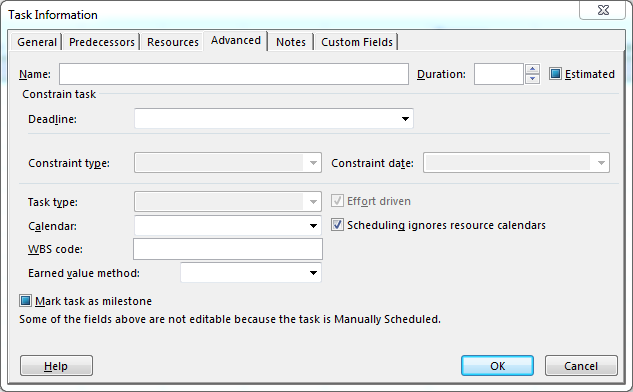
\includegraphics[width=10cm]{img/General.PNG}
	\caption{Task General Tab}
	\label{fig:General}
\end{figure}

\begin{figure}
	\centering
		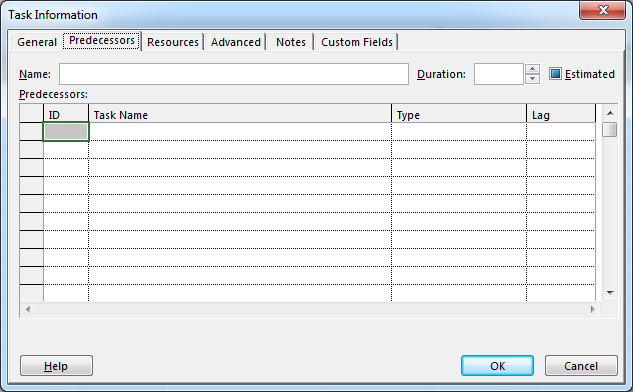
\includegraphics[width=10cm]{img/Predecessors.PNG}
	\caption{Task Predecessors Tab}
	\label{fig:Predecessors}
\end{figure}

\begin{figure}
	\centering
		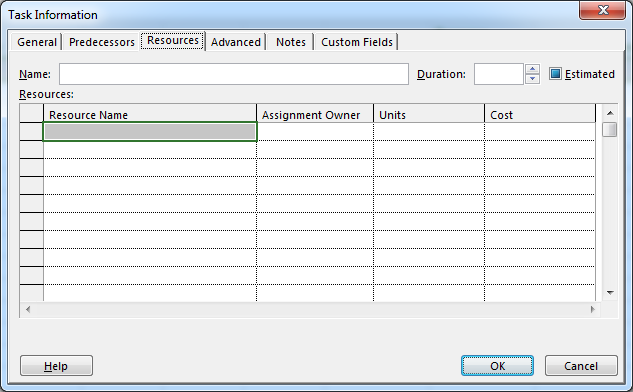
\includegraphics[width=10cm]{img/Resources.PNG}
	\caption{Task Resources Tab}
	\label{fig:Resources}
\end{figure}

\begin{figure}
	\centering
		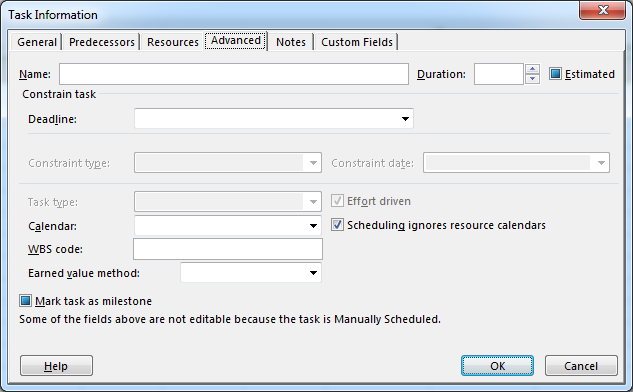
\includegraphics[width=10cm]{img/Advanced.PNG}
	\caption{Task Advanced Tab}
	\label{fig:Advanced}
\end{figure}

\begin{figure}
	\centering
		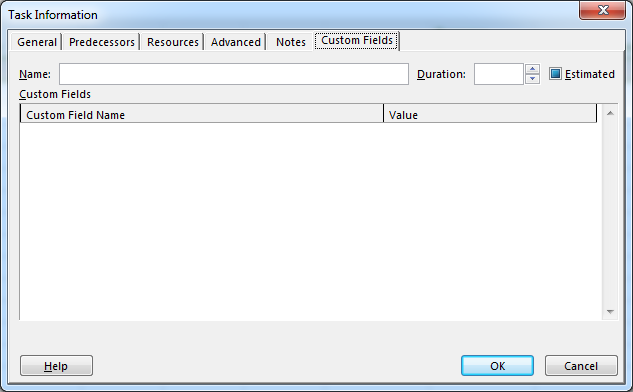
\includegraphics[width=10cm]{img/Custom.PNG}
	\caption{Task Custom Fields Tab}
	\label{fig:Custom}
\end{figure}

\begin{figure}
	\centering
		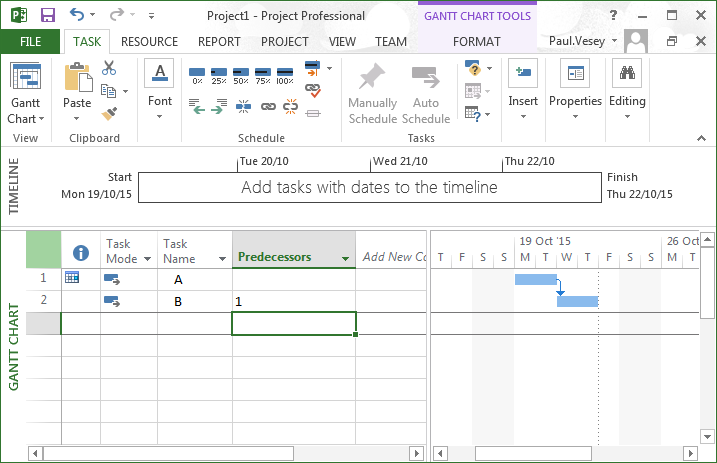
\includegraphics[width=10cm]{img/FS.PNG}
	\caption{Finish-Start Relationship}
	\label{fig:FS}
\end{figure}

\begin{figure}
	\centering
		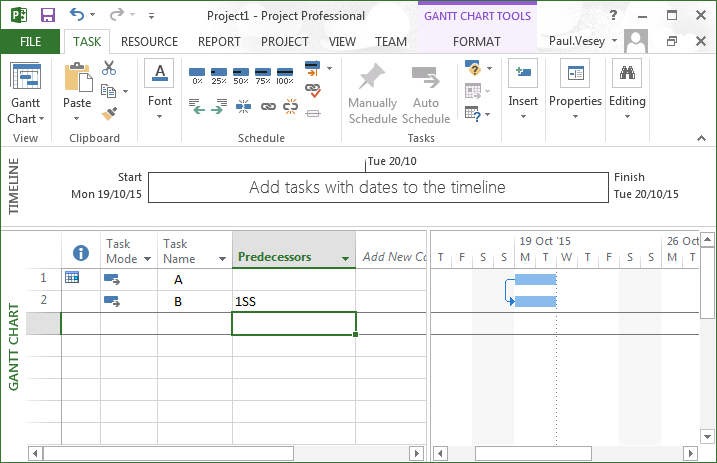
\includegraphics[width=10cm]{img/SS.PNG}
	\caption{Start-Start Relationship}
	\label{fig:SS}
\end{figure}

\begin{figure}
	\centering
		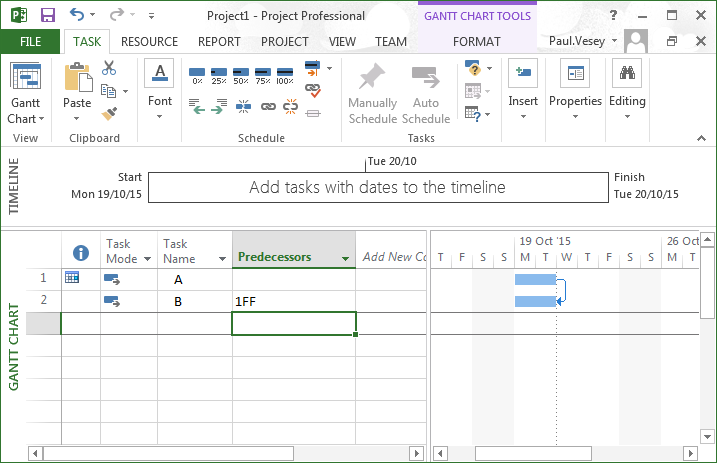
\includegraphics[width=10cm]{img/FF.PNG}
	\caption{Finish-Finish Relationship}
	\label{fig:FF}
\end{figure}

\begin{figure}
	\centering
		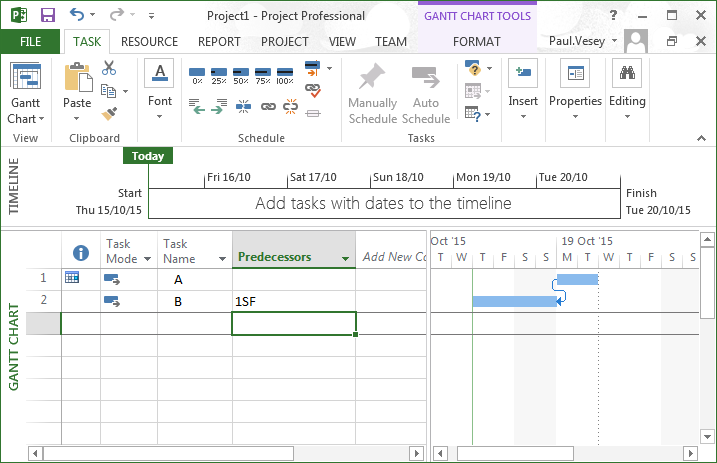
\includegraphics[width=10cm]{img/SF.PNG}
	\caption{Start-Finish Relationship (DO NOT USE)}
	\label{fig:SFl}
\end{figure}



\end{document}